\section{Технический проект}
\subsection{Общая характеристика организации решения задачи}

Необходимо спроектировать и разработать СУБД, которая должна способствовать хранению и фильтрации данных.

Система управления базами данных представляет собой набор взаимосвязных функций и макроссов, которые отвечают за работу с таблицами. БД представляет собой хэш-таблицу со структурами таблиц пользователей, которые имеют такие поля: название, списки колонок, списки столбцов.

\subsection{Обоснование выбора технологии проектирования}

На сегодняшний день информационный рынок, поставляющий программные решения в выбранной сфере, предлагает множество продуктов, позволяющих достигнуть поставленной цели – разработки СУБД.

\subsubsection{Описание используемых технологий и языков программирования}

В процессе разработки СУБД используются программные средства и языки программирования. Каждое программное средство и каждый язык программирования применяется для круга задач, при решении которых они необходимы.

\subsubsection{Язык программирования Lisp}

Lisp - это один из старейших языков программирования высокого уровня, созданный в 1958 году Джоном Маккарти. Первоначально он был разработан для исследований в области искусственного интеллекта и быстро стал одним из самых популярных языков для решения задач, связанных с обработкой данных, символическим вычислением и логическим выводом.

\paragraph{Основные особенности языка программирования Lisp}

\begin{enumerate} 
\item Символьная обработка. 
\item Простота синтаксиса.
\item Поддержка функционального программирования.
\item Макросы.
\item Множество диалектов.
\end{enumerate}

\subsection{Диаграмма компонентов и схема обмена данными между файлами компонента}

Диаграмма компонентов описывает особенности физического представления разрабатываемой системы. Она позволяет определить архитектуру системы, установив зависимости между программными компонентами, в роли которых может выступать как исходный, так и исполняемый код. Основными графическими элементами диаграммы компонентов являются компоненты, интерфейсы, а также зависимости между ними. На рисунке \ref{comp:image} изображена диаграмма компонентов для проектируемой системы. 

\begin{figure}[ht]
\center{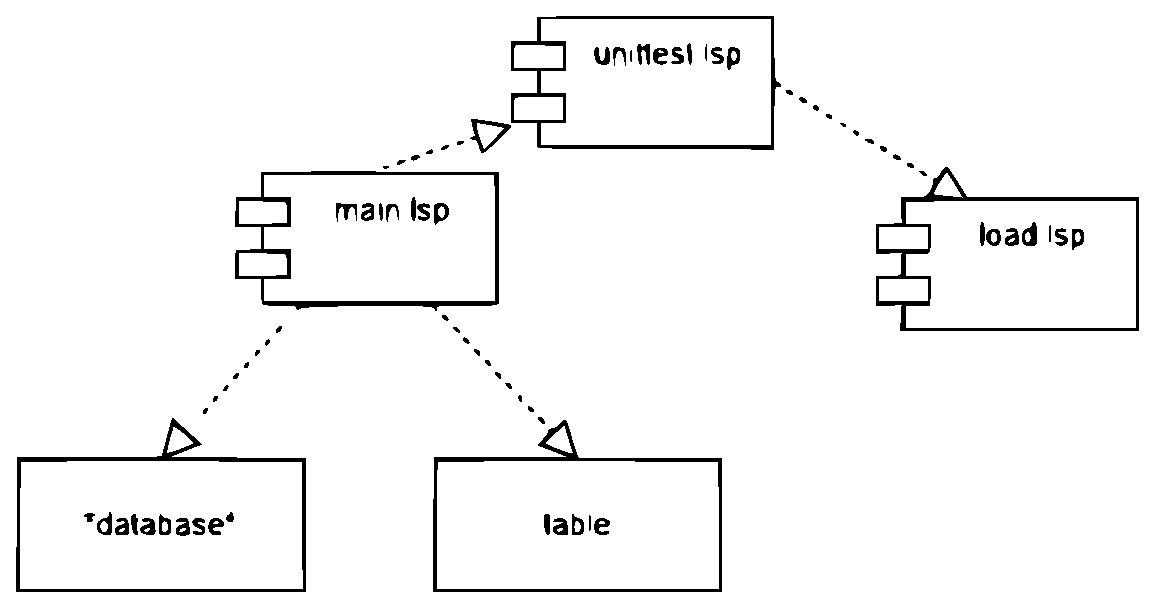
\includegraphics[width=1\linewidth]{comp}}
\caption{Диаграмма компонентов}
\label{comp:image}
\end{figure}
